% Chapter 1
\chapter{Introducción general} % Main chapter title

\label{Chapter1} % For referencing the chapter elsewhere, use \ref{Chapter1} 
\label{IntroGeneral}

%----------------------------------------------------------------------------------------

% Define some commands to keep the formatting separated from the content 
\newcommand{\keyword}[1]{\textbf{#1}}
\newcommand{\tabhead}[1]{\textbf{#1}}
\newcommand{\code}[1]{\texttt{#1}}
\newcommand{\file}[1]{\texttt{\bfseries#1}}
\newcommand{\option}[1]{\texttt{\itshape#1}}
\newcommand{\grados}{$^{\circ}$}

%----------------------------------------------------------------------------------------

%\section{Introducción}
En este capítulo se introducen conceptos asociados al uso de Internet de las Cosas (IoT) en invernaderos, la motivación del cliente y cuál es el estado del arte. Asimismo, se explican los objetivos y el alcance establecidos.
% el concepto de vivero inteligente, se exponen la motivación del cliente, sus objetivos y expectativas, como así también una evaluación del estado del arte.
%----------------------------------------------------------------------------------------
\section{Introducción}
\label{Introducción}

%El término Internet de las Cosas (en inglés, \textit{Internet of Things} abreviado IoT) hace referencia a la extensión de conectividad de red y capacidad de cómputo a objetos, sensores y otros dispositivos que normalmente no son considerados computadoras. A través de estos mecanismos pueden generar, intercambiar y consumir datos con mínima intervención humana.\citep{iotOverview}.


El término Internet de las Cosas (IoT) se refiere a escenarios en los que la conectividad de red y la capacidad de cómputo se extienden a objetos, sensores y artículos de uso diario que habitualmente no se consideran computadoras, permitiendo que estos dispositivos generen, intercambien y consuman datos con una mínima intervención humana \citep{iotOverview}.
IoT tiene una amplia variedad de campos de aplicación, entre los cuales se destaca la agricultura inteligente aplicada a invernaderos.

Los invernaderos modernos son sistemas de cultivo intensivo diseñados para alcanzar una alta eficiencia y productividad. Debido a su capacidad para mantener las condiciones ambientales en niveles óptimos o subóptimos, facilitan la producción de plantas a lo largo de todo el año en forma independiente a las condiciones climáticas externas \citep{HistoryofControlledEnvironmentHorticultureGreenhouses}.

La aplicación de IoT a invernaderos ha demostrado una mejora sustancial en la eficiencia de la gestión de los cultivos al mismo tiempo que ha logrado acelerar la producción y reducir sus costos \citep{IoTparaInvernaderos}. Además de las ventajas mencionadas, los invernaderos pueden impactar de forma positiva a los entusiastas de la jardinería, ya que proporcionan beneficios tanto físicos como anímicos especialmente durante las temporadas invernales o de baja temperatura \citep{GreenHousesForHomeOwnersAndGardeners}. 


\section{Motivación}
\label{Motivación}

El cliente de este proyecto es un jubilado reciente que decidió comenzar una nueva vida en una finca rural. Su intención es convertir la propiedad en una residencia sustentable, capaz de producir diferentes tipos de plantas: por un lado, hortalizas para abastecer el consumo familiar y por otro, especies de árboles para reforestación. 

Para lograrlo con mínima intervención humana en el proceso, surge la necesidad de instalar un invernadero que automatice el control de los cultivos y además tenga la capacidad de adaptar las condiciones climáticas y de riego a los diversos tipos de plantas a sembrar. 

 
En la figura \ref{fig:imgInvernadero} se observa un vivero hogareño típico de producción y dimensiones similares al propuesto.




\begin{figure}[htpb]
\centering 
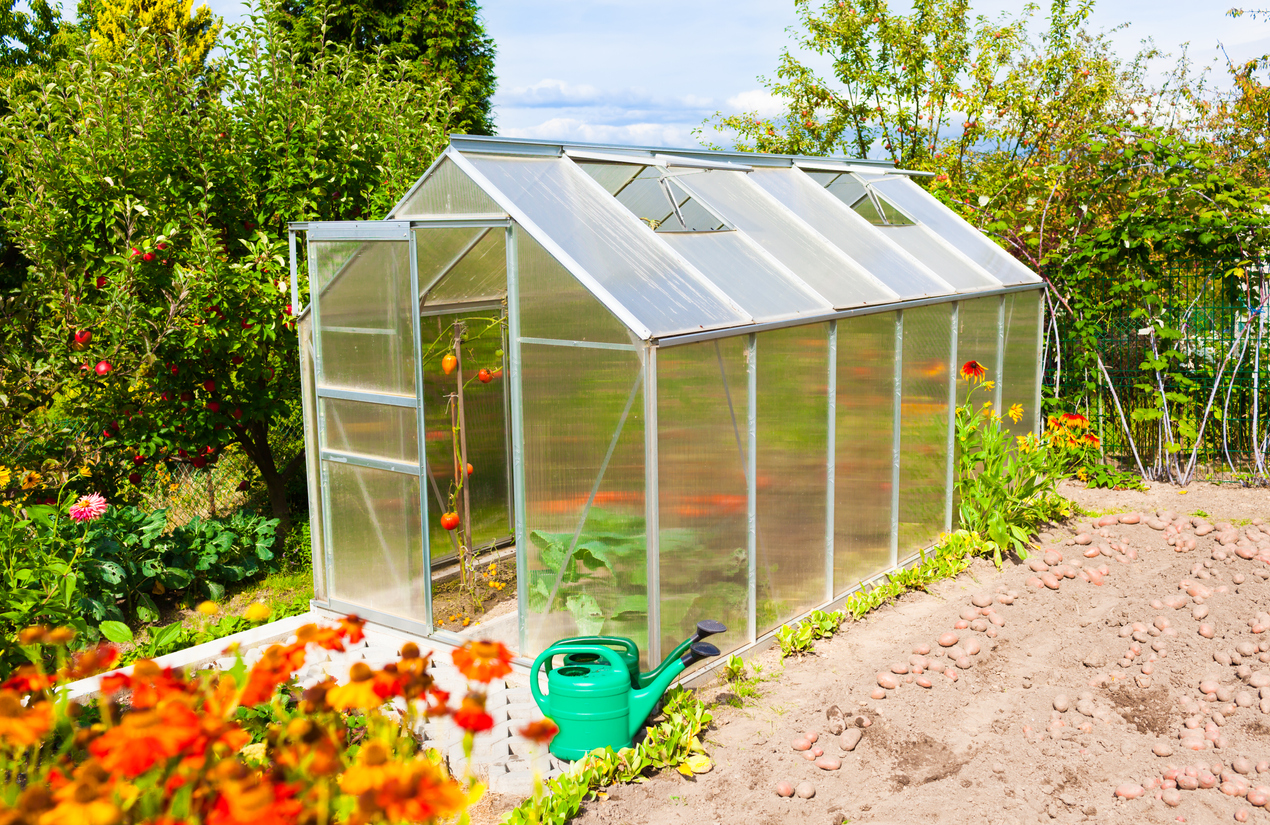
\includegraphics[width=.7\textwidth]{../Figures/invernadero1.jpg}
\caption[Invernadero hogareño]{Invernadero hogareño\protect\footnotemark.}
\label{fig:imgInvernadero}
\end{figure}


\footnotetext{Imagen bajo licencia de \url{https://www.istockphoto.com/}}



%----------------------------------------------------------------------------------------

\section{Estado del arte}
\label{sec:Estado del arte}

Los invernaderos son estructuras diseñadas para controlar y proteger a las plantas del clima y otros factores ambientales adversos. Tradicionalmente, la temperatura, humedad e iluminación se controlaban de forma manual, lo que requería una gran cantidad de mano de obra y recursos. 

Sin embargo, debido a los avances tecnológicos, se ha popularizado el desarrollo de invernaderos capaces de ajustar las condiciones ambientales mediante el uso de sensores, actuadores y controladores. Estos dispositivos responden en función de configuraciones preprogramadas o a partir de datos en tiempo real.  

Así el despliegue de este tipo de sistemas, denominados invernaderos inteligentes, se ha extendido enormemente en los últimos años debido a la eficiencia obtenida durante la producción y al incremento en la resiliencia de los cultivos \citep{agrofacto}. 


Algunas posibles aplicaciones de IoT en viveros incluyen:

\begin{itemize}
	\item Monitoreo y control del clima: distintos sensores miden la temperatura, humedad, iluminación y otros factores ambientales en el invernadero, para que luego diferentes actuadores automáticos ajusten el clima y creen las condiciones óptimas para el crecimiento de las plantas.

    \item Riego a demanda: la medición continua de la humedad del suelo permite activar sistemas de riego automatizados para mantener los niveles óptimos de humedad. Se logra así reducir el desperdicio de agua y disminuir los costos asociados.

    \item Seguimiento del crecimiento de las plantas: los sensores IoT pueden medir el crecimiento de las plantas y proporcionar información útil para la gestión del cultivo. Esto puede ayudar a identificar problemas de crecimiento temprano y a tomar medidas que eviten problemas mayores a futuro.

    \item Control de plagas y enfermedades: monitorear sus niveles en el vivero y activar sistemas de control cuando se detecten problemas ayuda a reducir el uso de pesticidas y otros productos químicos.
    
   \item  Fertirrigación: el sistema puede administrar fertilizantes o nutrientes al suelo de forma optimizada y precisa a través del riego, en base a configuraciones acordes a la plantación en curso o mediante sensores que midan las características del agua, el pH o la conductividad eléctrica entre otras.

    \item Automatización de tareas: los sistemas IoT pueden automatizar muchas tareas en el vivero, como la siembra, el trasplante y la recolección de plantas. Esto puede reducir los costos de mano de obra y mejorar la eficiencia de la producción.
\end{itemize}    

En la figura \ref{fig:imgInvernaderoInteligente} se representa un invernadero inteligente con sus respectivos sensores y actuadores.

\begin{figure}[htpb]
\centering 
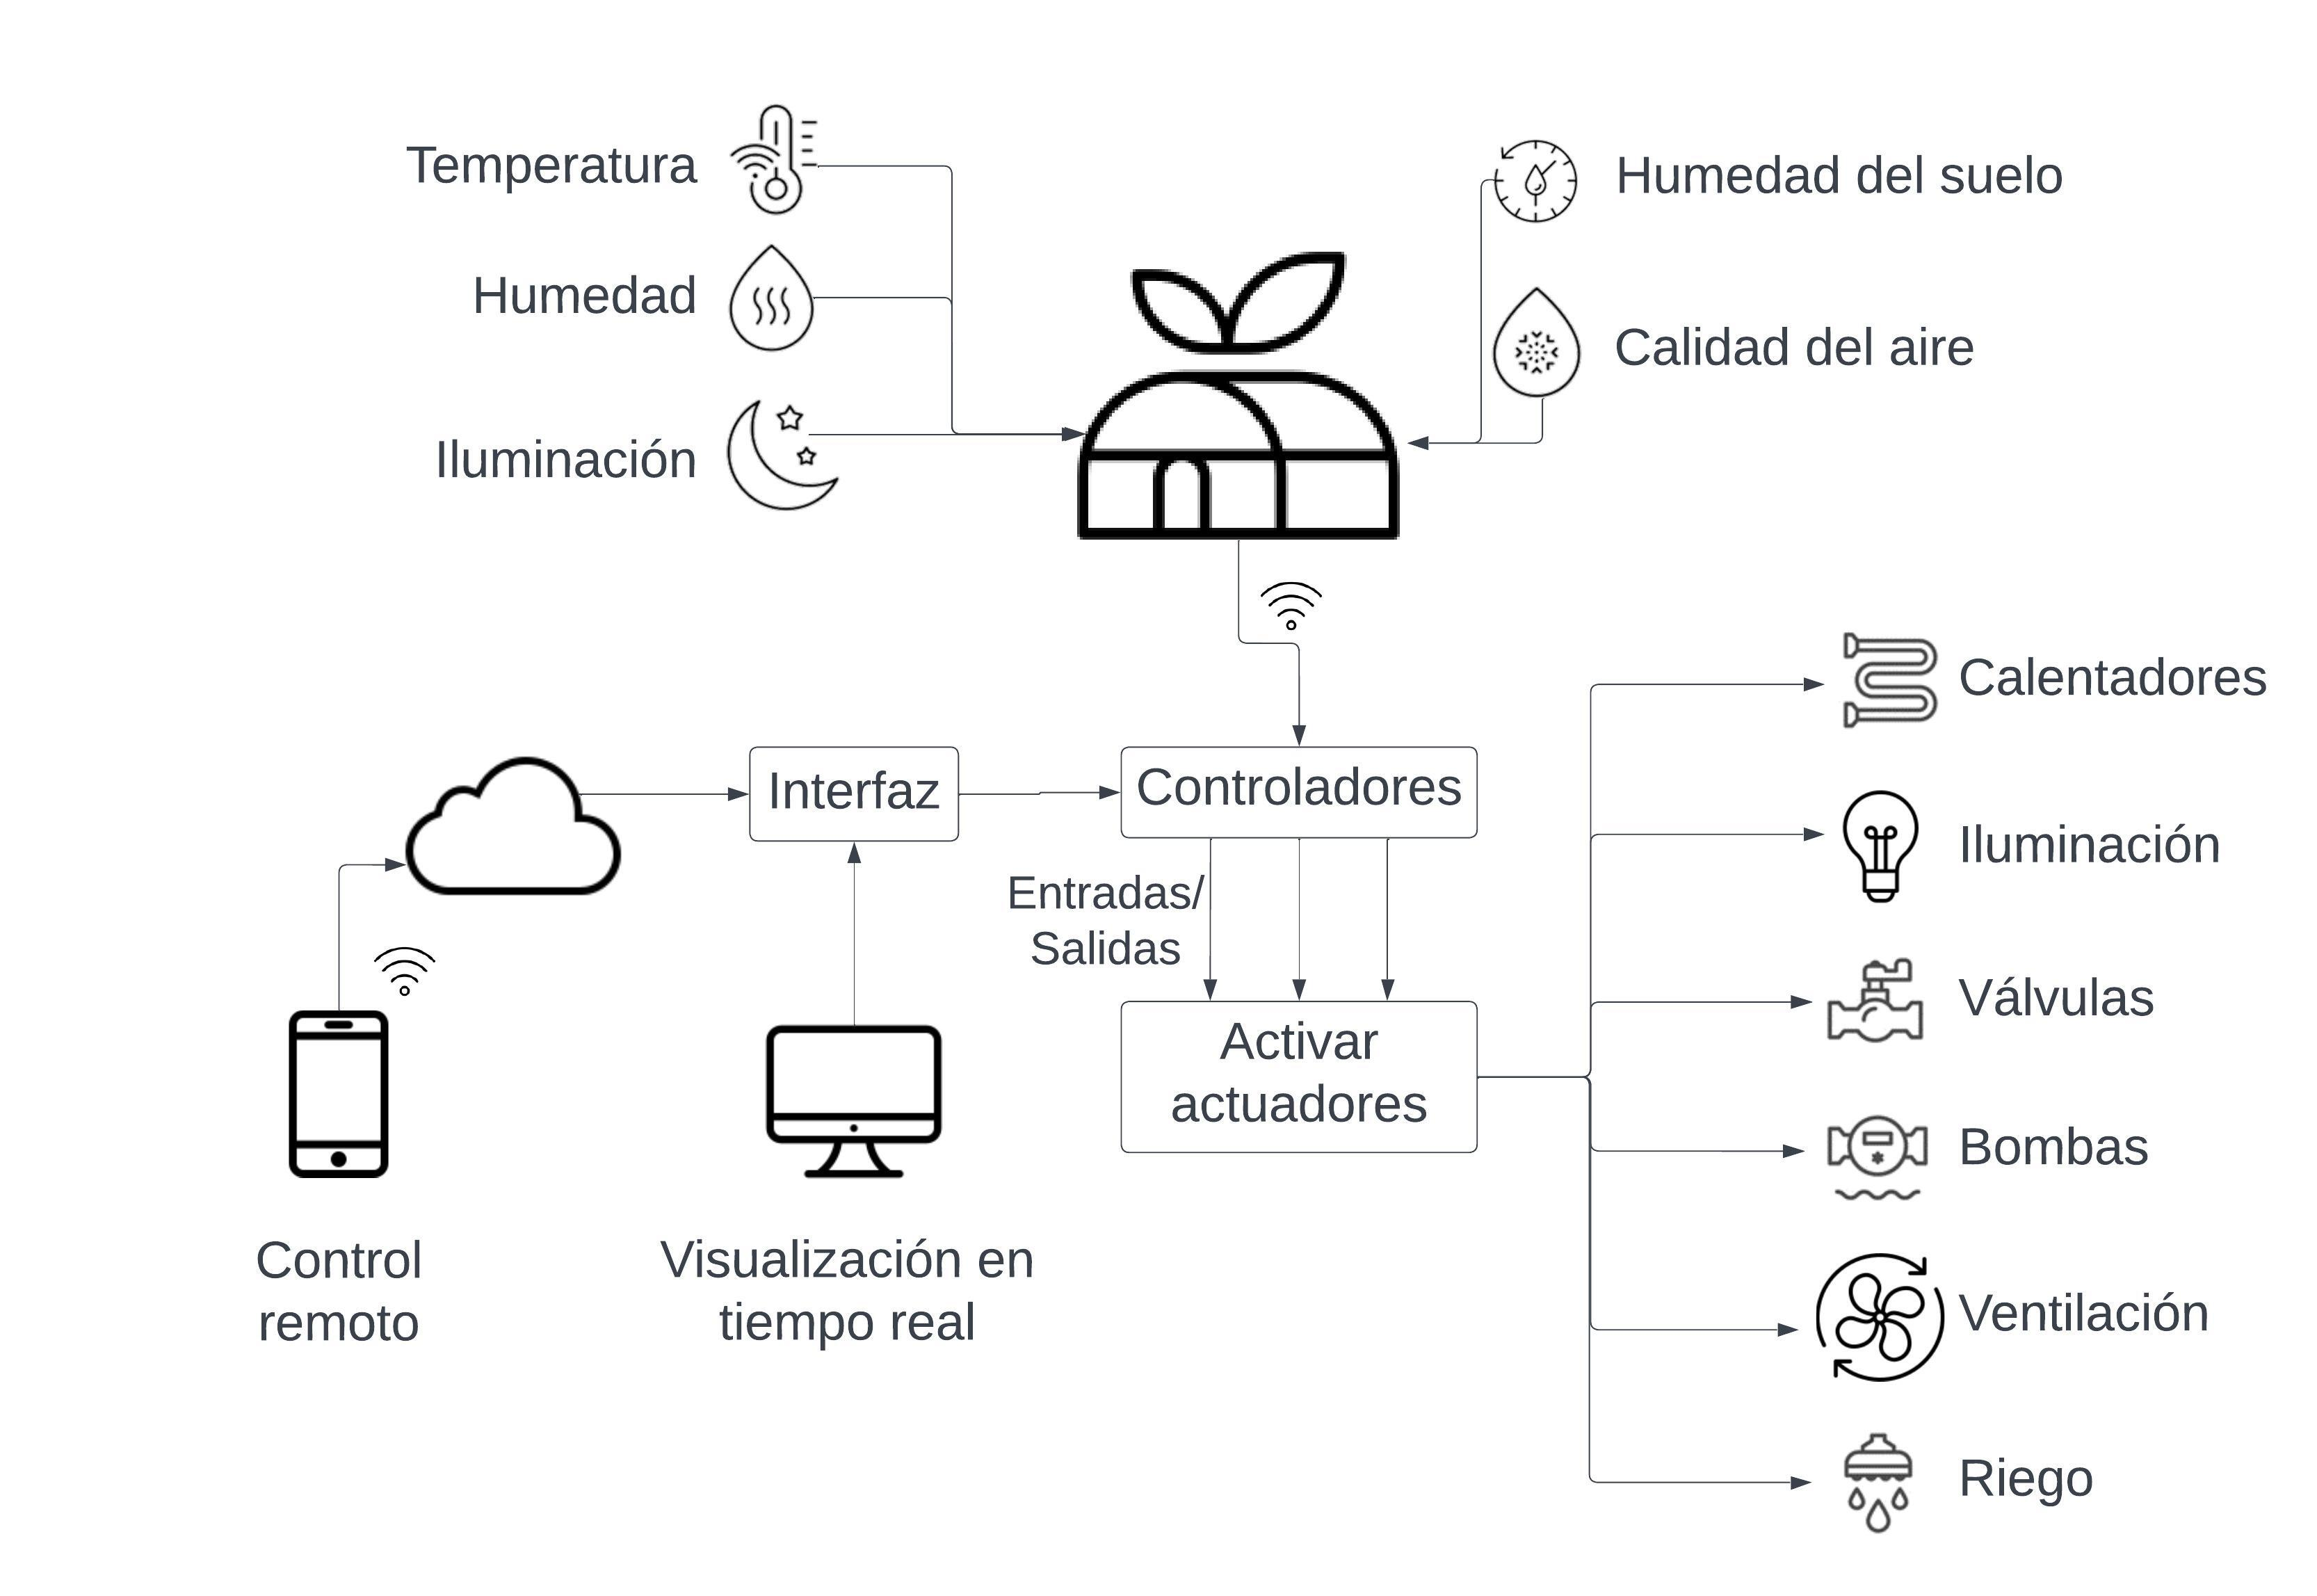
\includegraphics[width=.9\textwidth]{../Figures/SmartGreenhouse.jpeg}
\caption[Invernadero inteligente controlado por IoT]{Invernadero inteligente controlado por IoT\protect\footnotemark.}
\label{fig:imgInvernaderoInteligente}
\end{figure}

\footnotetext{Imagen adaptada de \textit{Internet of Things Empowered Smart Greenhouse Farming} \citep{9051987}.}




En el mercado internacional se encuentran diferentes proveedores que ofrecen soluciones para el desarrollo de invernaderos inteligentes. A la hora de comparar distintas opciones es necesario considerar los niveles de automatización requeridos, la facilidad de uso y las opciones de personalización. Adicionalmente, se debe considerar el costo y la compatibilidad con la infraestructura existente. 

En la tabla \ref{tab:vendors} se observa una breve comparación entre los principales proveedores comerciales de servicios. Allí se observa que en general las soluciones presentadas ofrecen características similares siendo el costo el mayor diferenciador.



\begin{table}[h]
\centering
\caption[Análisis del estado del arte]{Análisis del estado del arte.}

\begin{tabular}{lcccccc} 
\toprule
%\textbf{Funcionalidad} & \textbf{Priva []} & \textbf{Hortimax []} & \textbf{Argus Controls []} &\textbf{Grodan []} & \textbf{Heliospectra []} & \textbf{Growlink []}\\
\textbf{Funcionalidad} & \textbf{Argus Controls \citep{arguscontrol}} &\textbf{Grodan \citep{grodan}} & \textbf{Growlink \citep{growlink}}\\

\midrule
Gestión de clima    & Sí & Sí & Sí \\
Control de riego    & Sí & Sí & Sí \\
Fertirrigación      & Sí & Sí & Sí \\
Gestión de energía  & No & Sí & Si \\
Tamaño de mercado   & Grande & Grande & Pequeño \\
Costo               &  \$\$\$\$ & \$\$\$ &  \$\$ \\
\bottomrule
\hline
\end{tabular}
\label{tab:vendors}
\end{table}

\pagebreak
A manera de ejemplo, algunas soluciones comerciales ofrecen kits que pueden costar más de USD 200 por sensor, con gastos adicionales asociados al transporte y almacenamiento de datos. De esta forma, las redes inalámbricas de sensores pueden llegar a requerir presupuestos mayores a USD 10 000 por invernadero \citep{digger:1}. Las figuras \ref{fig:grodan} y \ref{fig:growlink} muestran diferentes soluciones que se encuentran en el mercado. 

\begin{figure}[htb]
\centering 
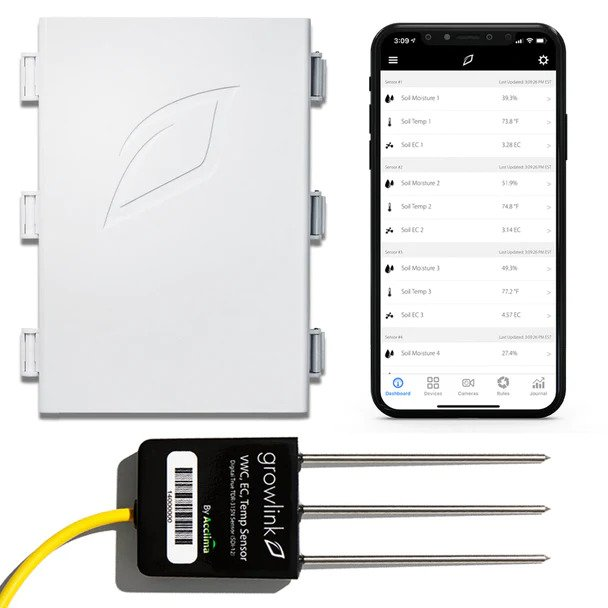
\includegraphics[width=.5\textwidth]{../Figures/growlink.jpg}
\caption[Sistema de control de irrigación de Growlink]{Sistema de control de irrigación de Growlink\protect\footnotemark.}
\label{fig:grodan}
\end{figure}
\footnotetext{Imagen bajo licencia de \url{https://www.growlink.com/}}


\begin{figure}[hb]
\centering 
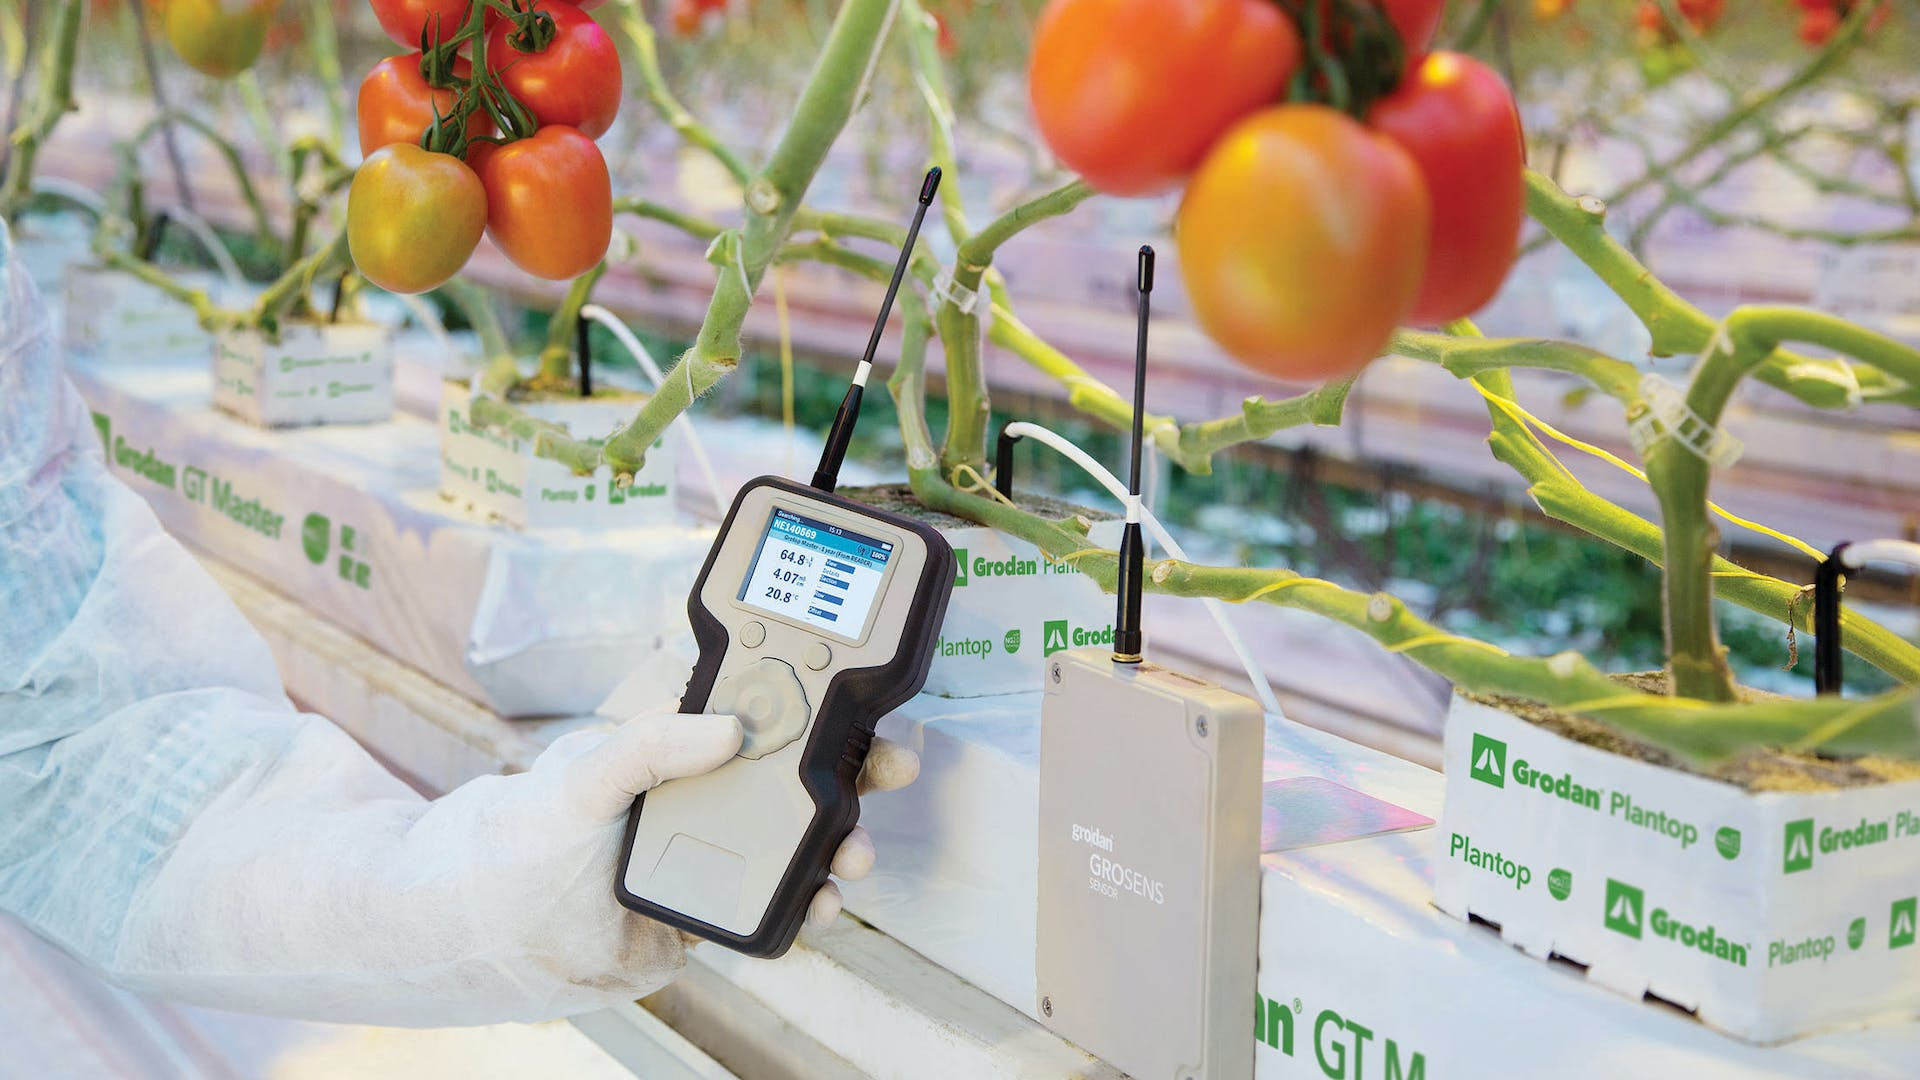
\includegraphics[width=.5\textwidth]{../Figures/grodan.jpg}
\caption[Sistema multisensor de Grodan]{Sistema multisensor de Grodan\protect\footnotemark.}
\label{fig:growlink}
\end{figure}


\footnotetext{Imagen bajo licencia de \url{https://www.grodan.com/}}

Una alternativa es utilizar kits de IoT como los provistos por Arduino \citep{arduino}, una plataforma de hardware y software de código abierto. Además, es necesario contar con una comunidad de usuarios que colaboren en el proceso de desarrollo. En contrapartida, para aplicar esta solución se requieren conocimientos de programación y electrónica no siempre disponibles para el cultivador promedio \citep{digger:1}. \\


%----------------------------------------------------------------------------------------

\section{Objetivos y alcance}
\label{sec:objetivos}

El propósito de este trabajo es el desarrollo de una plataforma capaz de controlar el clima y riego de un invernadero mediante el uso de sensores y actuadores. Estos dispositivos se comunican con una aplicación instalada en un servidor local que administra los parámetros y las alarmas del sistema.

Durante el proyecto se construyó un prototipo completo de invernadero con los siguientes elementos:
 
\begin{itemize}
	\item Aplicación para el monitoreo, control de dispositivos, gestión de alarmas y automatización.
	\item Control de usuarios, permisos y accesos a la plataforma.
	\item Interfaz gráfica para acceso y control de la plataforma.
	\item Análisis, investigación y elección del hardware para los sensores y actuadores.


\end{itemize}


El trabajo no incluyó:
\begin{itemize}
	\item Instalación en sitio de los sistemas desarrollados.
	\item Implementación de métodos de control basados en condiciones climatológicas externas.
	\item Desarrollo o implementación de modelos analíticos o predictivos de las condiciones del vivero.
	\item Diseño o instalación de conexiones que no sean por Wi-Fi (LTE/5G). 
	
\end{itemize}